%%%%%%%%%%%%%%%%%%%%%%%%%%%%%%%%%%%%%%%%%%%%%%%%%%%%%%%%%%%%%%%%%%%%%
% LaTeX Template: Project Titlepage Modified (v 0.1) by rcx
%
% Original Source: http://www.howtotex.com
% Date: February 2014
% 
% This is a title page template which be used for articles & reports.
% 
% This is the modified version of the original Latex template from
% aforementioned website.
% 
%%%%%%%%%%%%%%%%%%%%%%%%%%%%%%%%%%%%%%%%%%%%%%%%%%%%%%%%%%%%%%%%%%%%%%

\documentclass[12pt]{report}
%\usepackage[a4paper]{geometry}
\usepackage{graphicx}
\graphicspath{{./}}
%\usepackage{fancyhdr}
%\usepackage{lastpage}
%\usepackage{graphicx, wrapfig, subcaption, setspace, booktabs}
%\usepackage[T1]{fontenc}
%\usepackage[font=small, labelfont=bf]{caption}
%\usepackage{fourier}
%\usepackage[protrusion=true, expansion=true]{microtype}
%\usepackage[english]{babel}
%\usepackage{sectsty}
%\usepackage{url, lipsum}


\newcommand{\HRule}[1]{\rule{\linewidth}{#1}}
%%\onehalfspacing
\setcounter{tocdepth}{5}
\setcounter{secnumdepth}{5}

%-------------------------------------------------------------------------------
% HEADER & FOOTER
%-------------------------------------------------------------------------------
%\pagestyle{fancy}
%\fancyhf{}
%\setlength\headheight{15pt}
%\fancyhead[L]{BE PROJECT}

%-------------------------------------------------------------------------------
% TITLE PAGE
%-------------------------------------------------------------------------------

\begin{document}

\title{ \normalsize \textsc{IEEE Zagazig Branch-CS}
		\\ [2.0cm]
		\HRule{0.5pt} \\
		\LARGE \textbf{\uppercase{OPINION ON JAVASCRIPT FRAMEWORKS}}
		\HRule{2pt} \\ [0.5cm]
		\normalsize  \vspace*{5\baselineskip}}

\date{}

\author{
		Ahmed Anwar \\
        Guided By - Ahmed Moustafa\\ }

\maketitle
\newpage
There are many frontend frameworks. every one try to solve some problem or not (some are reduntant) but generally that is why they exist (probably also because of market as they have to make new ones to keep frontend developers constantly learning so they stay in business). Anyway as I have to learn a framework that would be Vue as it is built to be fast and also no company is pushing it like react \& Facebook. Vue also has a nice feature it is extermely lightweight in fact that is why it was made in the first place. I personally don't have enough experience to recommend or to decide what is the best but Vue is used a lot, it is the second one after react.
\begin{figure}[h]
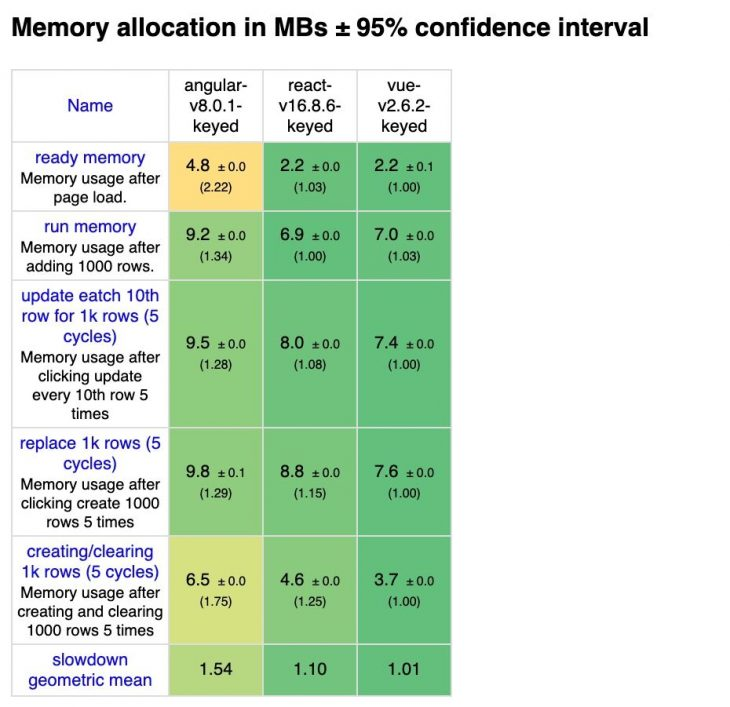
\includegraphics[width=\textwidth]{memory-allocation-comparison}
\end{figure}
\begin{figure}[h]
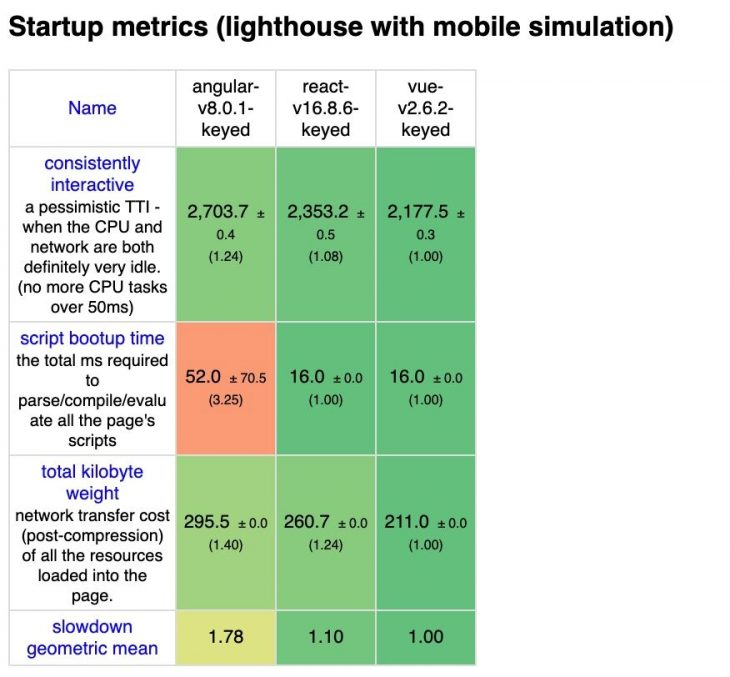
\includegraphics[width=\textwidth]{startup-time-comparison}
\end{figure}
\begin{figure}[h]
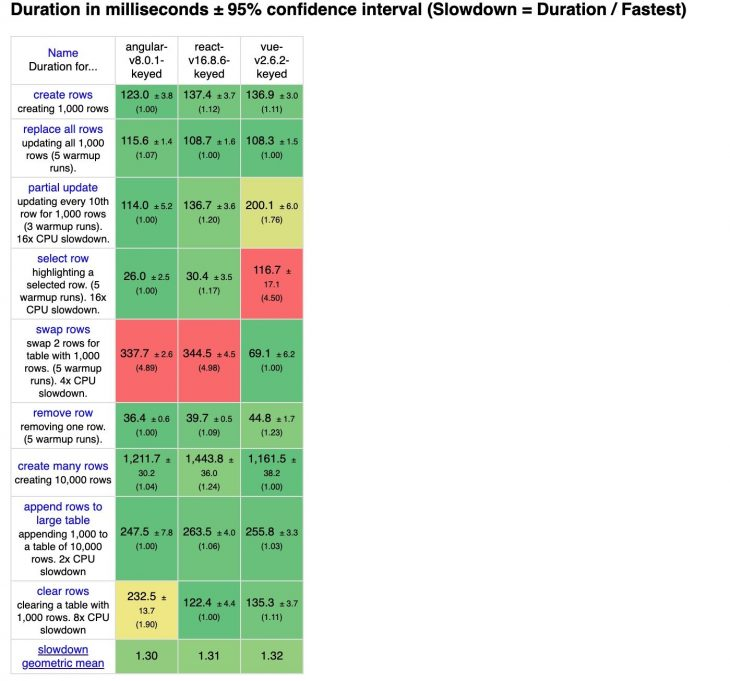
\includegraphics[width=\textwidth]{dom-manipulation-comparison}
\end{figure}
\end{document}
